\section{Parallel Rheobase Determination}\label{sec:parallel-rheobase}
In the preceding section, I discussed determination of the rheobase of a model as one of most computationally expensive steps in evaluating a given set of model parameters. 

\subsection{Why is the Rheobase Important?}
The rheobase is defined as the minimum current required to elicit at least one action potential.
In slice physiology experiments, this usually means a square pulse of somatically-injected current lasting for a fixed amount of time, for example $500 ms$.
The rheobase not only characterizes the excitability of a cell, but it also serves as a landmark or anchor for computing many other features of a cell's suprathreshold behavior.
For example, once the rheobase is known, one can compute a so-called "FI curve" -- the number or frequency of action potentials in response to a given amount of injected current -- at fixed multiples of the rheobase, providing a compact summary of excitability.
Both the Allen Institute and the Blue Brain Project use such rheobase-linked excitability measures.
The rheobase current can also be used to compute features of spike waveforms.
These features may vary with the amount of injected current, because the rising phase of an action potential may include both sodium current and pipette currents.
By using the rheobase current, this latter confound is minimized because the patch pipette current is roughly offset by outward currents (were the pipette current any less, the outward currents would have prevented a spike, by the definition of rheobase).
Consequently, action potential waveform features like threshold, width, and height are often performed at the rheobase current.

\subsection{How is the Rheobase Determined?}
Determining the rheobase involves repeated application of a more general algorithm that runs one simulation to determining the number of action potentials evoked by a particular magnitude and duration of somatic current injection.
Because the rheobase value partitions suprathreshold stimulus amplitudes from subthreshold ones, its determination can be accelerated by treating as a search tree problem.
In a search tree, the search space is adaptively narrowed between two endpoints until a target is identified.
For the rheobase, this means asking (1) "What is maximum current injected so far that resulted in zero spikes?" and (2) "What is the minimum current so far that resulted in one or more spikes?" and then running a simulation at some current amplitude in between those two values (e.g. halfway between in the case of a binary search tree).

\subsubsection{Serial rheobase determination}
The procedure above can be run in serial (i.e one simulation after another) until the rheobase is narrowed down to an acceptably narrow range, e.g. +/- 1 pA.
The initial search begins with no knowledge of any minimum suprathreshold or maximum subthreshold current amplitudes, so I use the starting range 300 pA to -100 pA, respectively.
A binary search is applied within this space, with additional code to handle edge cases outside this range.
Ignoring those edge cases, such a binary search requires $log_2(I/i)$ simulations, where $I$ is the range being searched (here, 400 pA) and $i$ is the resolution of the solution (here, 1 pA).
Thus, ~9 simulations are required to obtain the rheobase using this binary search strategy.

\subsubsection{Parallel rheobase determination}
This process can be accelerated by running simulations in parallel.
While each step of the search requires knowledge of the outcomes of the previous simulations (and so there can be no parallelism across steps, other than brute force parallel search of the entire range of currents, which is extremely inefficient), it is possible to parallelize within each step.
A binary search partitions the search space in two by simulating a current injection at $(sub+super)/2$ pA, where $sub$ is the previous maximum subthreshold current, and $super$ is the previous minimum suprathreshold current.
The value $(sub+super)/2$ pA either does or does not produce a spike, leading to its value being used to update either $super$ or $sub$, respectively.
The search space is cut in half, so this simulation effectively generates one additional bit of information about the amplitude of the rheobase.
This repeats ~9 times until all 9 bits of uncertainty (from the initial 400 pA) range have been eliminated.
Parallelism accelerate this by applying an N-ary search (rather than a binary search), where N is the number of parallel processes, and N+1 the number of regions of current amplitude to search.
This is described in Figure \ref{fig:rheobase}.
Consider the initial 400 pA range.
With only one thread, this range is bisected and a simulation run at it midpoint $(-100 pA + 300 pA)/2 = 100 pA$.
With seven threads, this range can be octo-sected, with concurrent simulations run at each of seven values, i.e. ${-50, 0, 50, ..., 300, 350}$ pA.
The highest of these seven value that produces a spike is assigned to $sub$ and the lowest that does not to $super$, resulting in the search space now being restricted to only one of these 50 pA wide regions.
This is $1/8$ as a wide as the initial space, so 3 bits of information about the rheobase have been obtained.
This parallel process is then repeated serially (i.e. octo-section of the new 50 pA region, octo-section of the ensuing 6.25 pA region, etc.), until the rheobase has been determined.
Because 3 bits of information are obtained in every step instead of 1 bit, the search is 3x faster.
In general, the parallel N-ary approach is $log_2(N+1)$ faster than the plain serial binary search approach, with speedup gain therefore growing logarithmically in the number of concurrent threads (usually, proportional to the number of CPU cores) being used.
As architectures with hundreds of cores are now common, speedups of 7-10 fold are achievable.

\begin{figure}    
  \begin{center}
  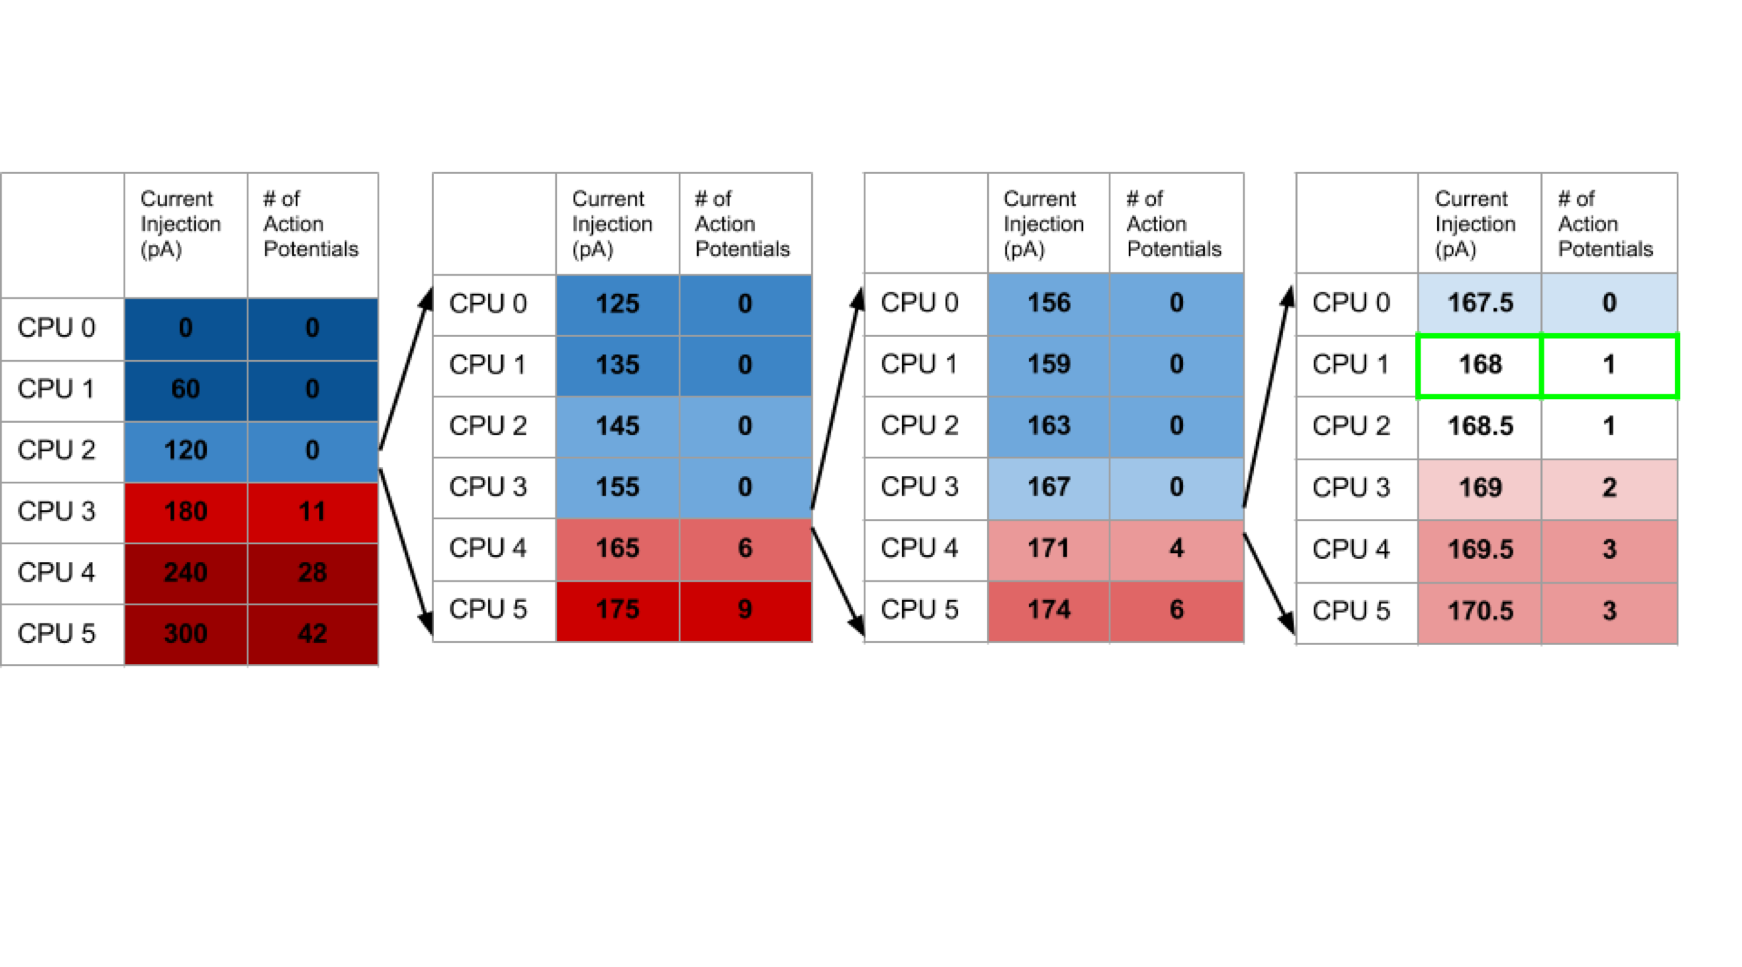
\includegraphics[width=0.9\linewidth]{{figures/rheobase_algorithm.png}}
    \caption[Parallel rheobase algorithm]{We developed a generic algorithm which took models, and found the minimal current injection value that would cause only one spike. The normal structure of this algorithm is a binary search, however we modified the algorithm so it would map onto multiple processors at once. This lead to significant speed ups for multicompartmental NEURON models}
    \label{fig:rheobase}
  \end{center}
\end{figure} 
    
\subsection{Practical application}
I benchmarked this approach using simulations of multi-compartment neuron models.
The parallel rheobase determination algorithm resulted in a significant speed up relative to the serial algorithm.
To amplify the effect, I also considered a scenario where one wants to learn the value of the rheobase with much more precision (down to small fractions of a pA), for example in studies of dynamics in the neighborhood of a bifurcation where all other state variables can be considered nearly unchanged in the sub- and suprathreshold scenarios.
To achieve such precision, i.e. for such a small value of $i$ $0.0001*pq.fA$, the number of simulations $log_2(I/i)$ may be ~20.
Since additional model features may require only a few additional simulations to extract, it is clear that in this scenario the rheobase completely dominates the bulk of the total simulation budget.

In this scenario, using only 16 threads (with a theoretical speedup of $log_2(16+1) ~ 4.09$), I achieved the following results:
\begin{verbatim}
NEURON simulation of multicompartmental model
Serial Rheobase determination: 18.7 s
Parallel Rheobase determination: 4.8 s
Speed up = 3.9x

Brian2 simulation of AdEx model
Serial Rheobase determination: 0.791 s
Parallel Rheobase determination: 0.259 s
Speed up = 3.0x
\end{verbatim}

The total speedup approached but fell a bit short of the theoretical speedup due to overhead in the parallel search algorithm itself.
As the complexity of each simulation increases, and as the number of CPU cores brought to bear increases, this overhead should become a vanishingly small fraction of the total rheobase determination time.

\subsection{Generalization to target spike counts}
This approach determining rheobase was also generalized into a more fundamental algorithm (\url{https://github.com/russelljjarvis/neuronunit/blob/master/neuronunit/tests/target_spike_current.py}) for determining the amplitude of current required to generate a target number of action potentials.
In other words, it can be used to invert points along a models ``F-I" function.

